% Created 2017-09-28 Jeu 14:17
\documentclass[11pt]{article}
\usepackage[margin=1.6in]{geometry}
\usepackage[T1]{fontenc}
%\usepackage{fixltx2e}
\usepackage{graphicx}
%\usepackage{longtable}
\usepackage{minted}
\usemintedstyle{colorful}
\setminted{fontsize=\footnotesize}
%\usepackage{wrapfig}
\usepackage{amsmath, amsthm}
%\usepackage{textcomp}
%\usepackage{marvosym}
%\usepackage{wasysym}
\usepackage{amssymb}
\usepackage{hyperref}
% Pour XeTeX
%\XeTeXdefaultencoding utf-8
\usepackage{fontspec}

% Appel usuel à des packages
\usepackage{listings}
\usepackage[frenchb]{babel}
\lstset{
  %frame=tb,
  language=C,
  aboveskip=2mm,
  belowskip=2mm,
  showstringspaces=false,
  columns=flexible,
  basicstyle={\scriptsize\ttfamily},
  numbers=none,
  numberstyle=\footnotesize\color{gray},
  keywordstyle=\color{blue},
  commentstyle=\color{dkgreen},
  stringstyle=\color{mauve},
  breaklines=true,
  breakatwhitespace=true
  tabsize=3
}

\newenvironment{absolutelynopagebreak}
  {\par\nobreak\vfil\penalty0\vfilneg
   \vtop\bgroup}
  {\par\xdef\tpd{\the\prevdepth}\egroup
   \prevdepth=\tpd}

\usepackage{color}
\definecolor{dkgreen}{rgb}{0,0.6,0}
\definecolor{gray}{rgb}{0.5,0.5,0.5}
\definecolor{mauve}{rgb}{0.58,0,0.82}

\theoremstyle{definition}
\newtheorem*{mydef}{Définition}

\theoremstyle{definition}
\newtheorem*{myrem}{Remarque}

\theoremstyle{definition}
\newtheorem*{myexemple}{Exemple}

\tolerance=1000
\setcounter{secnumdepth}{2}
\author{Borne, Isnel}
\date{}
\title{TP2: Etudes de performances}

\begin{document}

\maketitle

\section{Multiplication matrice/vecteur}
Nous étudions les gains de performances
liés à la parallélisation d'un algorithme de multiplication matrice/vecteur avec \texttt{OpenMP}.
Nous évaluons les performances du code suivant:
\begin{minted}[breaklines, numbersep=5pt, gobble=2, frame = lines, framesep=2mm]{c}
void mult_mat_vector_tri_inf (matrix M, vector b, vector c) {
  register int i ;
  register int j ;
  #pragma omp parallel for schedule(politique_ordonnancement, chunksize) private(i, j) num_threads(nb_thread)
  for(i=0; i<N; i++){
    for(j=N-1; j>=0; j--){
      c[i] += b[j] * M[i][j];
    }
  }
}\end{minted}
Nous nous intéressons en particulier à l'influence du choix de trois politiques d'ordonnancement (Statique, Dynamique, Guidé) ainsi que la valeur du paramètre \texttt{chunksize} sur le temps d'exécution de l'algorithme pour un nombre de fils d'exécution donné.
\subsection{Algorithme}
On considère une matrice $M$, de taille $N$ fixée à $1024$.
La directive \texttt{OpenMP} permet de répartir les itérations des boucles entre différents threads $T_1, T_2, ..., T_{nb\_threads}$. Un thread $T_i$, au cours de l'exécution du programme, se voit affecté successivement des "blocs" (\texttt{chunks}) d'itérations dont il aura la charge. La taille de ces "blocs" est spécifiée par le paramètre \texttt{chunksize}.

\subsection{Performances}
Notre machine possède 8 coeurs physiques et, grâce à l'hyperthreading, est capable d'exécuter deux threads par coeurs. Ainsi nous réalisons des mesures de temps d'exécution pour des valeurs de \texttt{nb\_thread} allant de 1 (exécution séquentielle) à 16. Pour chaque valeur de \texttt{nb\_thread} nous faisons ensuite varier la valeur de \texttt{chunksize} parmi $\{1, 2, 4, 10, 20, 50, 100, 500\}$.
\begin{myrem}
  Afin de pouvoir placer notre étude statistique dans le domaine d'application de la loi des grands nombres nous réalisons, pour chaque couple (\texttt{nb\_thread}, \texttt{chunksize}), la mesure du temps d'exécution $1000$ fois. La mesure du temps retournée par le programme est une moyenne sur 100 exécution de chaque fonction et nous lançons $10$ fois le programme pour chaque mesure. 
\end{myrem}
\subsubsection{Ordonnancement statique}
Avec la politique d'ordonnancement statique, la répartition des itérations entre les différents threads est figée avant l'exécution du programme. 
\begin{center}
  \begin{tabular} {c}
    \raisebox{-.5\height}{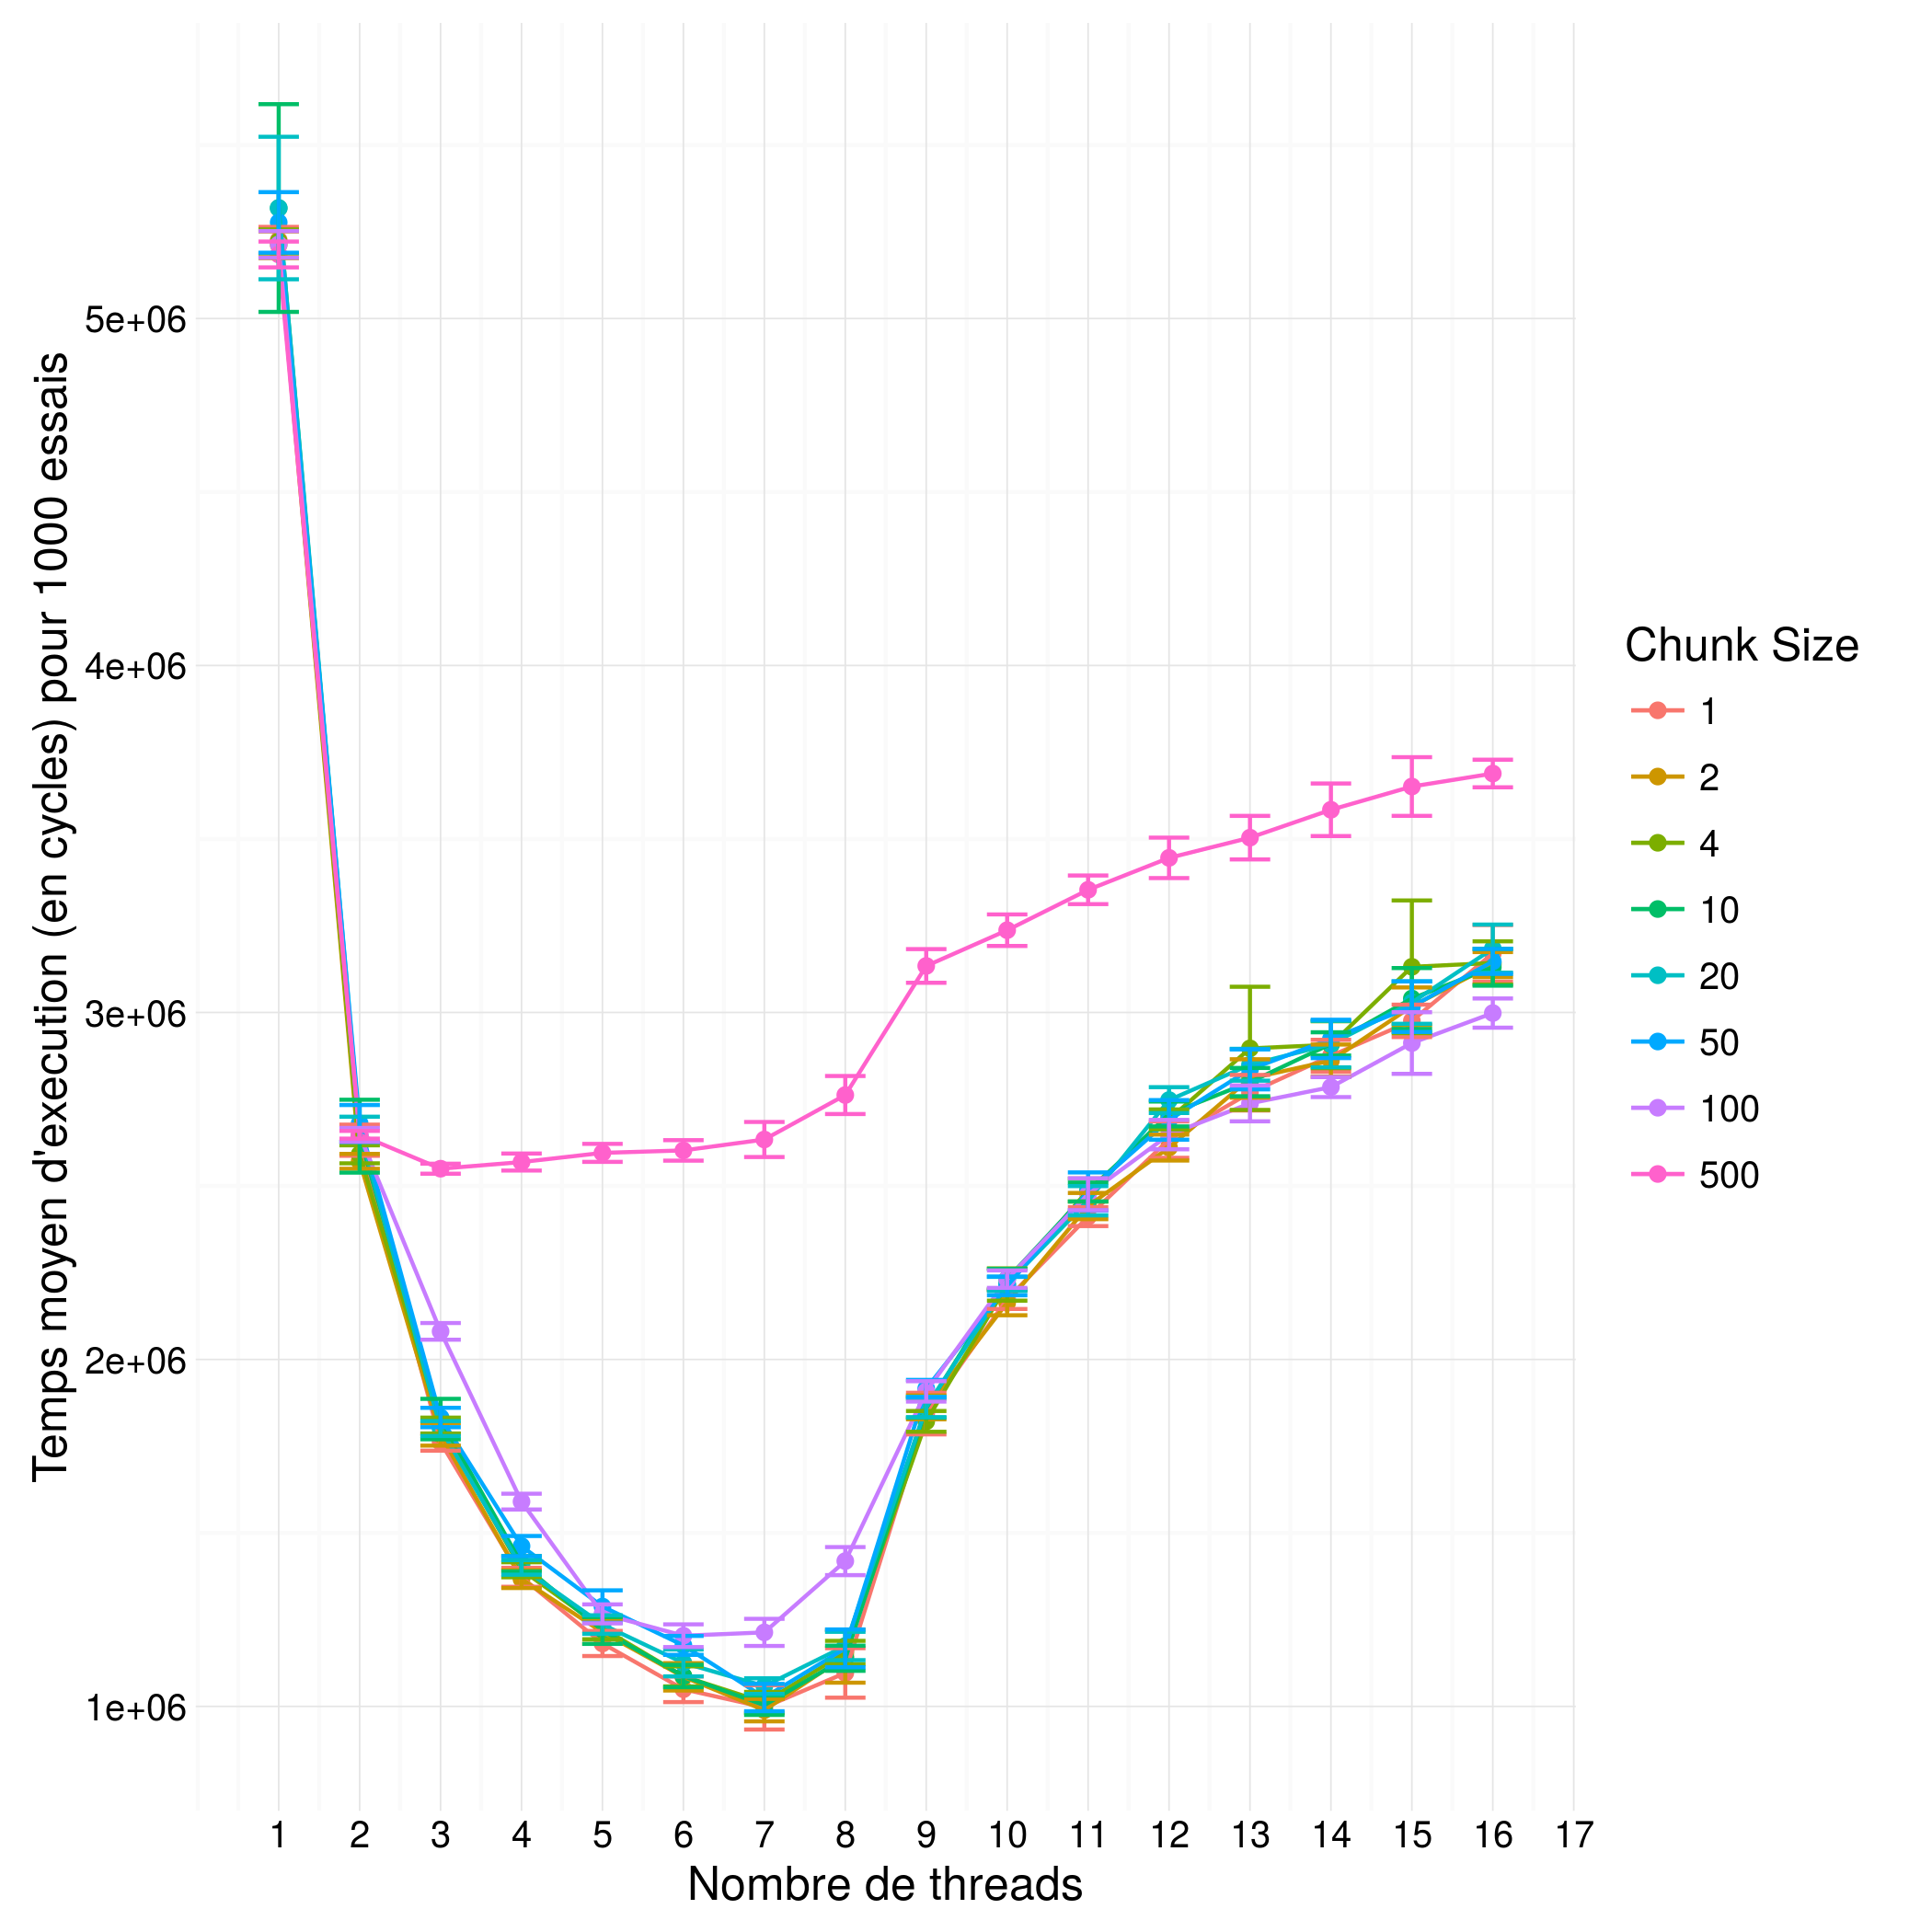
\includegraphics[keepaspectratio,scale=0.5]{./R/Images/Matrix_mult_algo2.png}}
  \end{tabular}
\end{center}
\begin{myrem}
Sur le graphique ci-dessus nous reportons pour chaque couple (\texttt{nb\_thread}, \texttt{chunksize})
l'écart type calculé pour nos mesures sous forme de "bâtonnet" vertical.
\end{myrem}
Nous observons bien le gain de performance apporté par la parallélisation. Avec deux threads, on met deux fois moins de temps qu'avec un seul. Au delà de deux threads on observe le comportement pathologique pour \texttt{chunksize} égal à 500 avec des performances nettement dégradées. Pour les autres valeurs de \texttt{chunksize}, le meilleur temps moyen est obtenu avec $7$ fil d'exécutions et on observe une très nette dégradation des performances au delà de cette valeur. Avec 9 thread on est deux fois moins efficace qu'avec 7.
Pour des valeurs situées en dessous d'une limite entre 100 et 500, \texttt{chunksize} n'a pas l'air d'affecter drastiquement les performances. 


\subsubsection{Ordonnancement dynamique}
Contrairement à l'ordonnancement statique, la répartition des itérations entre les threads n'est pas connue
avant l'exécution. Lorsqu'un thread finit d'exécuter sur son \texttt{chunk} d'itérations courant, il va
chercher, parmi les itérations pas encore affectées, un nombre \texttt{chunksize}, de nouvelles itérations sur lesquelles travailler. L'intérêt de cette politique se comprend quand le temps d'exécution varie beaucoup entre les différentes itérations.
Dans ces conditions, en mode statique, un thread pourrait se voir assigner tout le travail facile et attendre "les bras croisés"
que les autres finissent les tâches plus compliquées.
Dans notre application, il est raisonnable de supposer que les itérations sont de difficulté égale et qu'on ne
gagnera pas forcément à utiliser un ordonnancement dynamique. En effet, pour un thread, le fait d'aller chercher
de nouvelles itérations disponibles a un coût non négligeable. Le paramètre \texttt{chunksize} a précisément
pour but de limiter l'overhead induit par cette recherche.
\begin{center}
  \begin{tabular} {c}
    \raisebox{-.5\height}{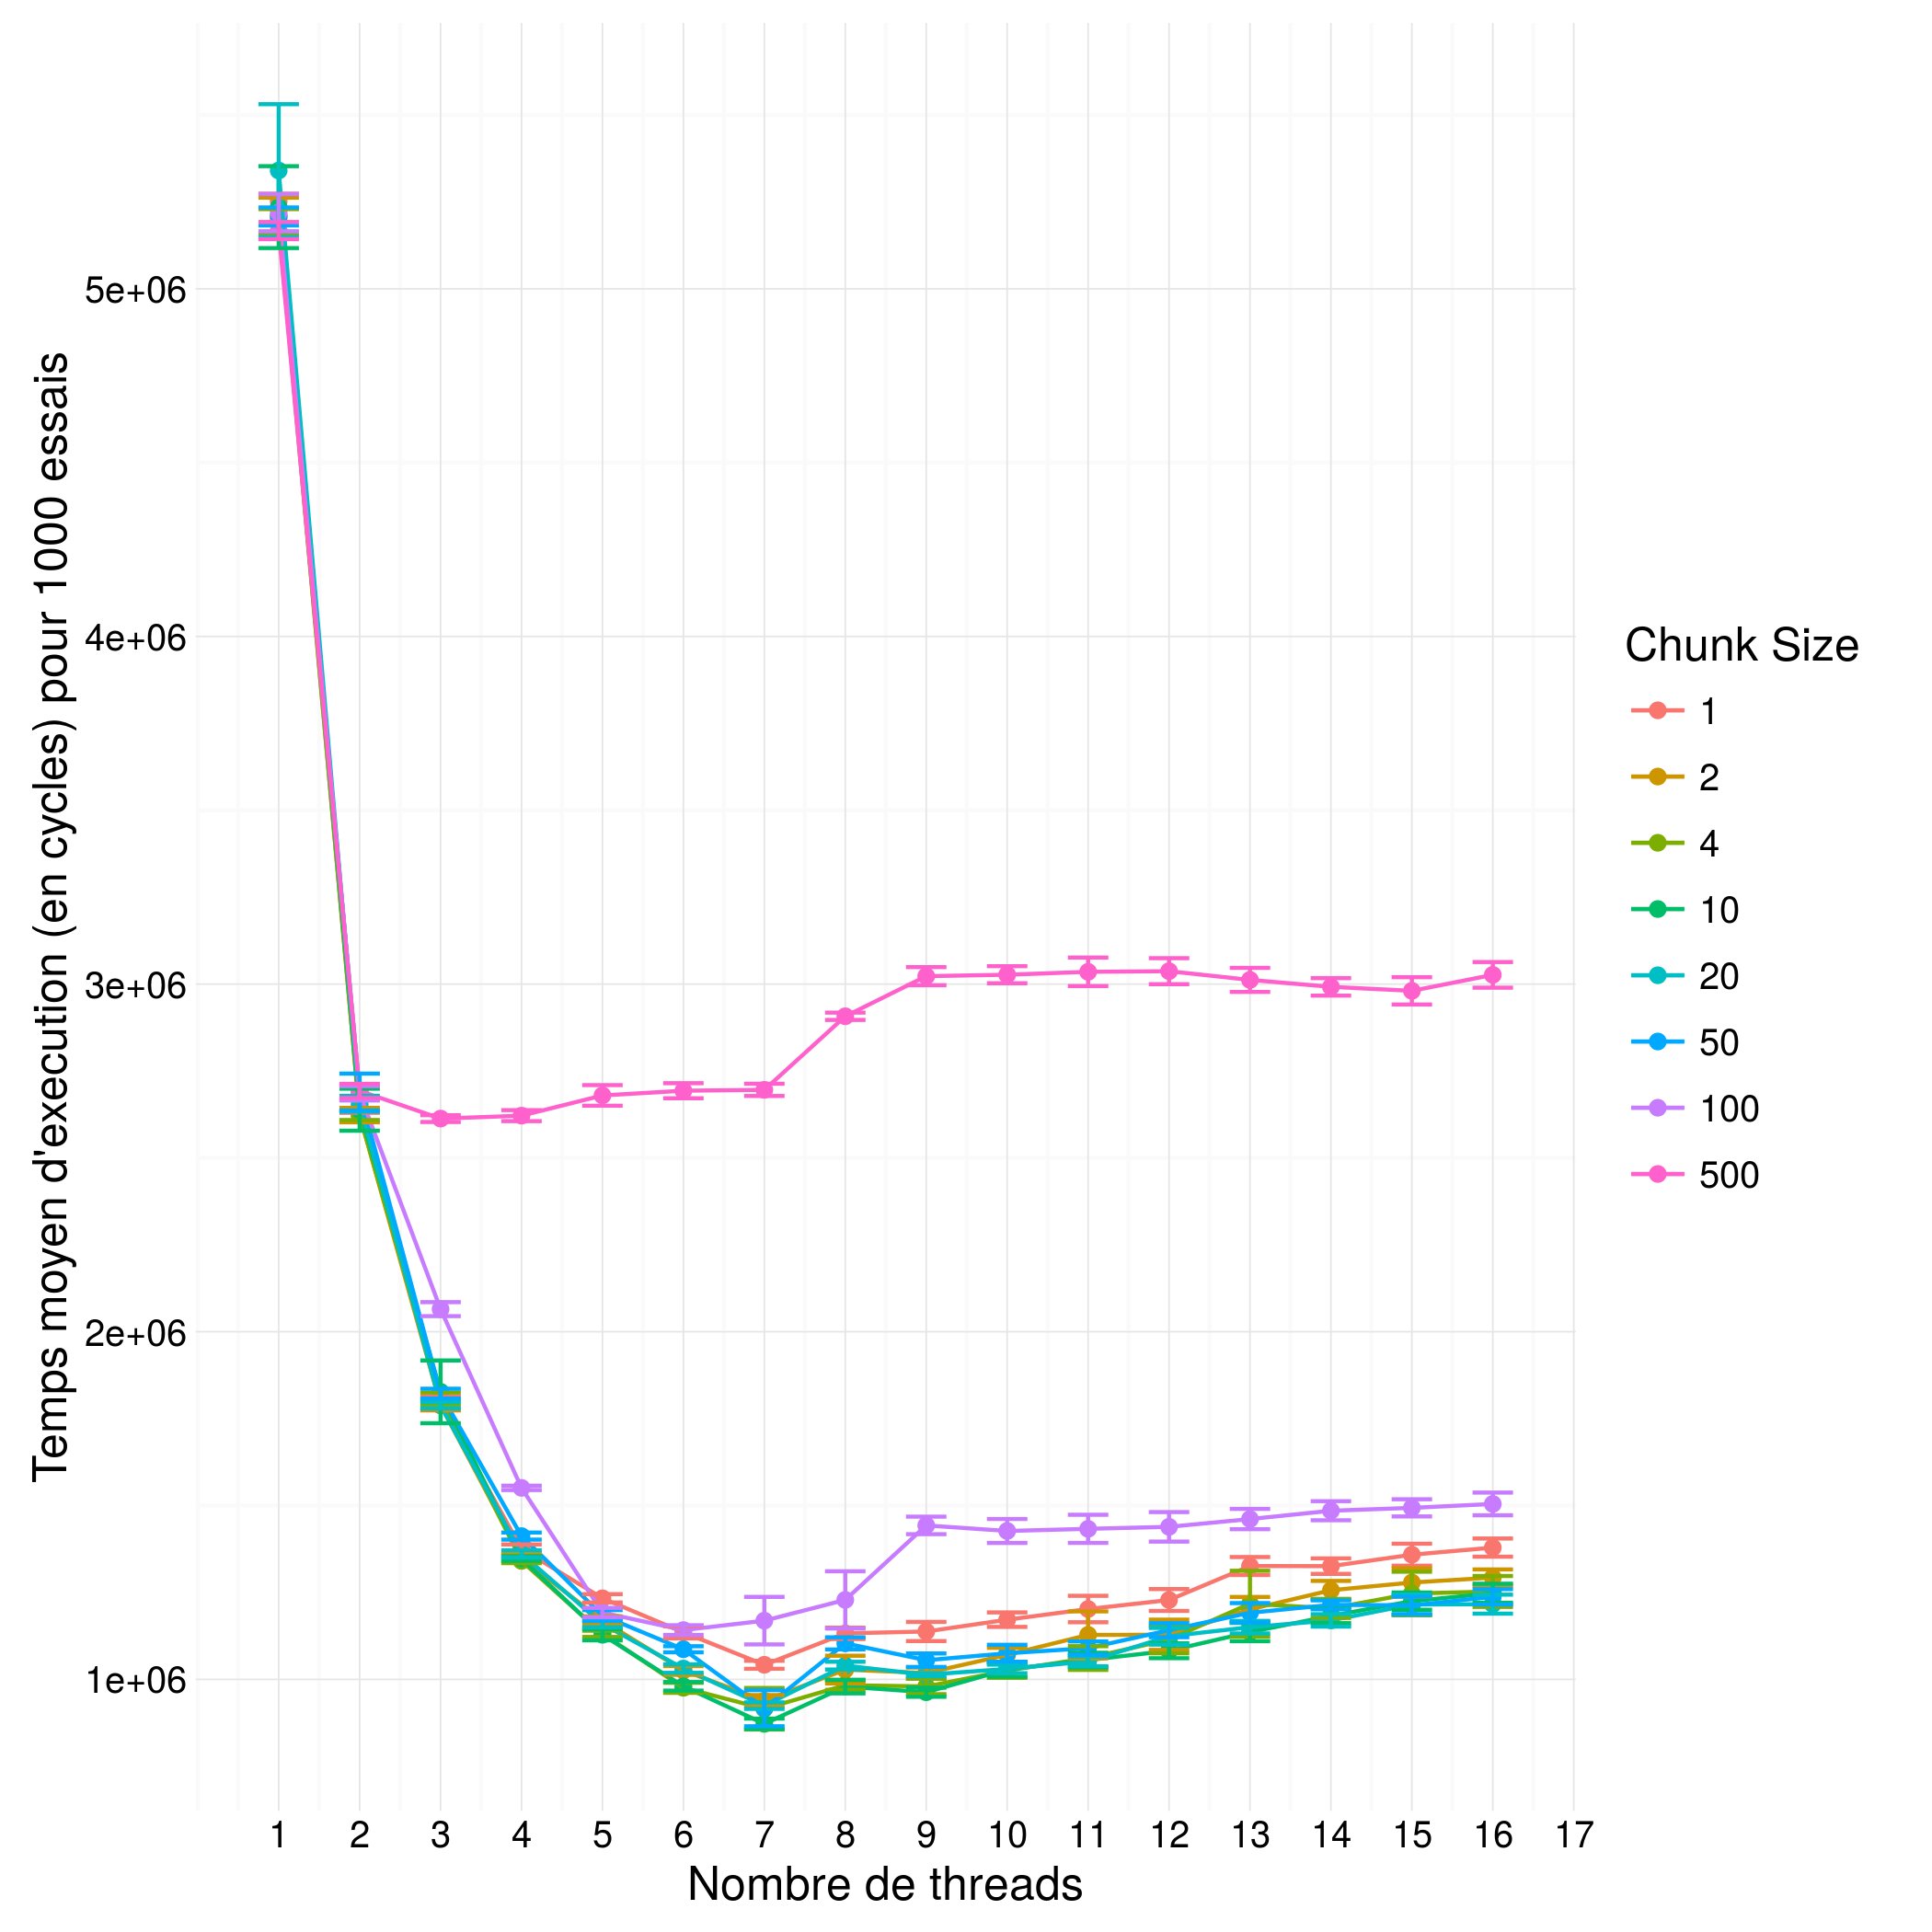
\includegraphics[keepaspectratio,scale=0.5]{./R/Images/Matrix_mult_algo3.png}}
  \end{tabular}
\end{center}
Nous observons ici aussi les gains de performances liés à la parallélisation et le même comportement pathologique pour
\texttt{chunksize} égal à 500. Les meilleurs temps d'exécution sont obtenus pour 7 threads et,
contrairement à l'ordonnancement statique, la dégradation des performances est peu marquée au delà de cette valeur.
On observe aussi l'influence de la taille des \texttt{chunk}. Ici le temps moyen mesuré avec \texttt{chunksize} égal
à 1 est moins bon que celui pour \texttt{chunksize} égal à 2, 4, 10, 20, 50. Aussi on met bien en évidence l'impact
de l'opération de recherche des itérations disponibles par un thread et de l'avantage d'affecter des blocs d'itération.
On remarque cependant que les gains observés avec des tailles de \texttt{chunk} > 1 sont d'un ordre de grandeur négligeable devant ceux observés par le passage d'un thread à deux thread par exemple. On voit aussi les effets négatifs que
peut avoir une taille de \texttt{chunk} trop grande.
\subsubsection{Ordonnancement guidé}

\begin{center}
  \begin{tabular} {c}
    \raisebox{-.5\height}{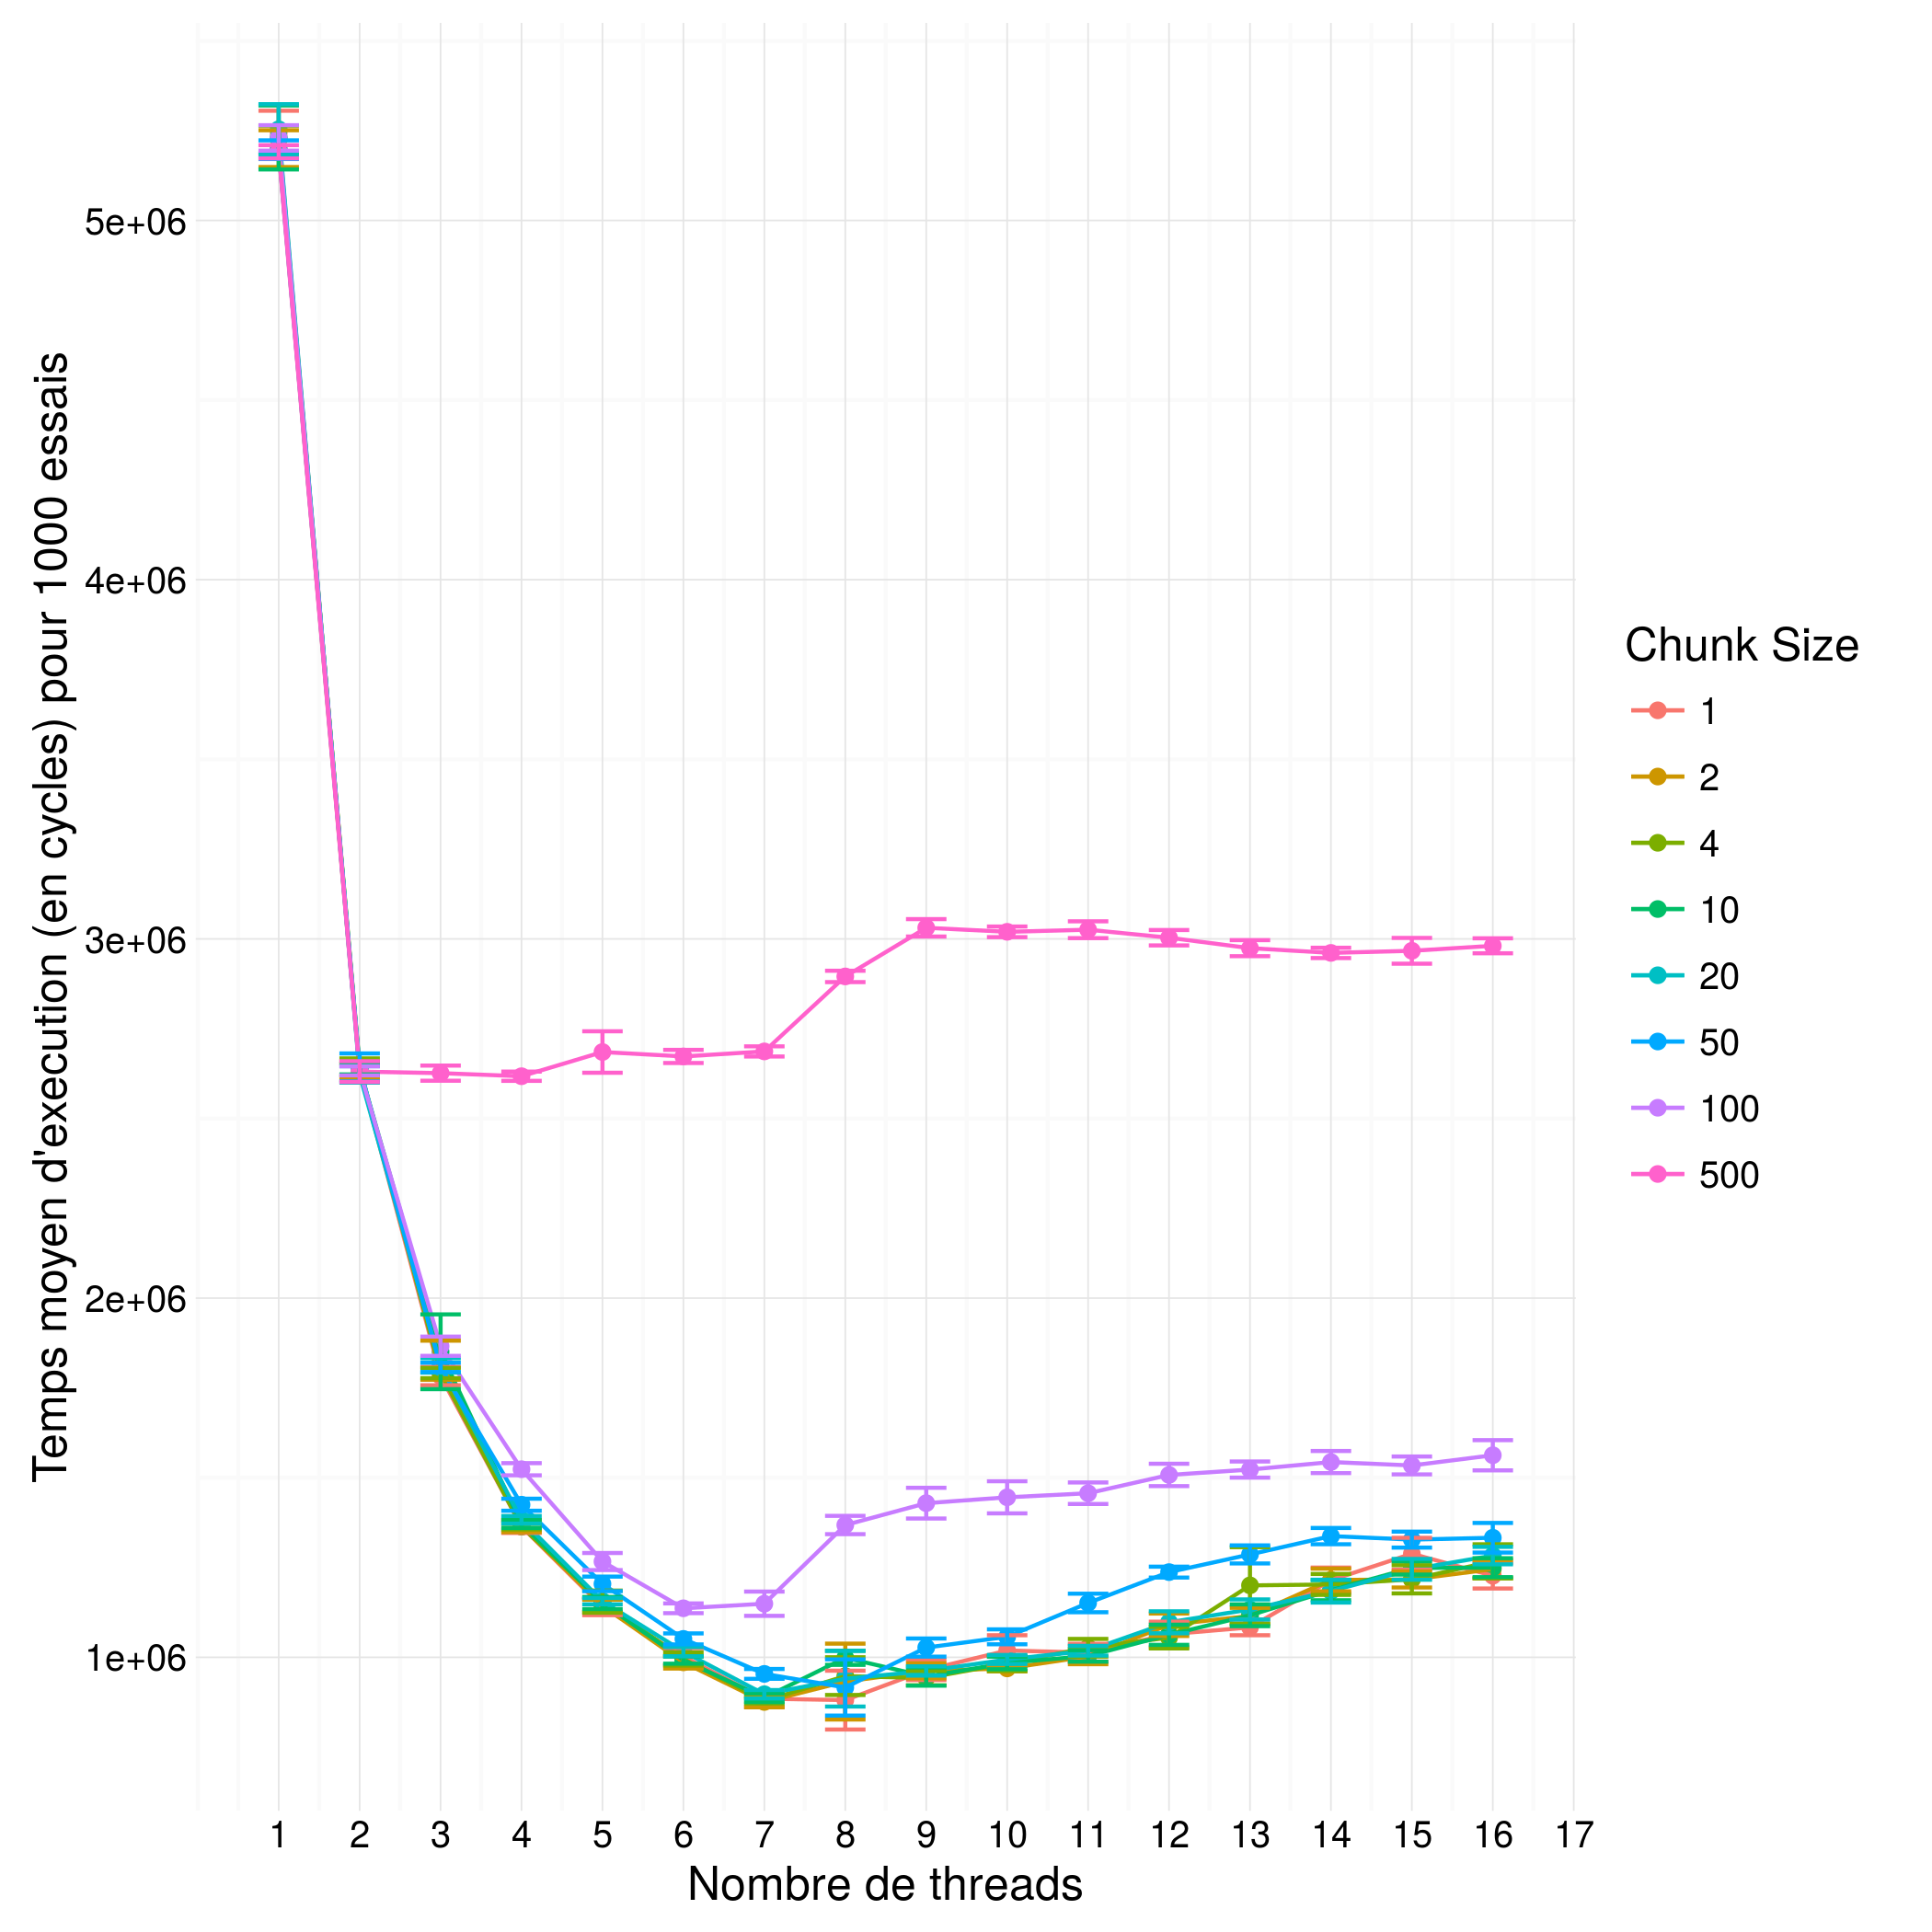
\includegraphics[keepaspectratio,scale=0.5]{./R/Images/Matrix_mult_algo4.png}}
  \end{tabular}
\end{center}

\subsubsection{Accélération}
Une autre représentation des performances peut-être faite en terme de facteur d'accélération.
l'accélération s'exprime comme le temps moyen de la version séquentielle d'un algorithme
divisé par le temps moyen de la version parallèle. On prends pour référence de temps d'exécution séquentiel, celui
de l'algorithme naïf de multiplication entre une matrice et un vecteur.
\begin{center}
  \begin{tabular} {c}
    \raisebox{-.5\height}{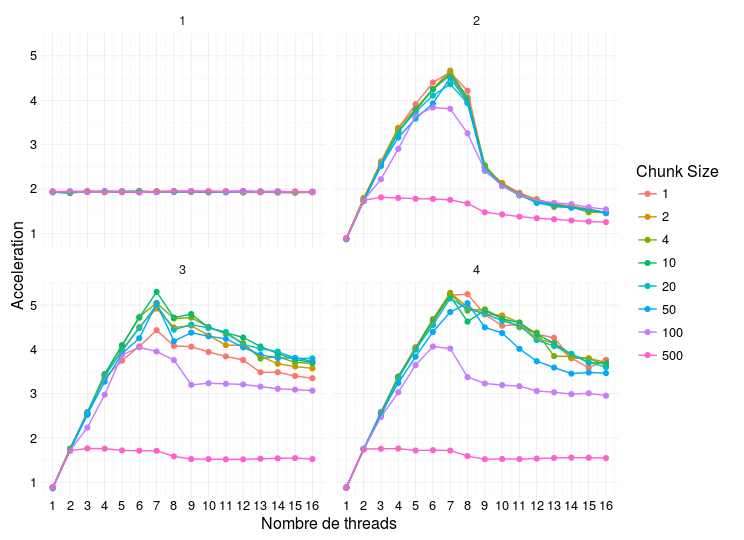
\includegraphics[keepaspectratio,scale=0.5]{./R/Images/Matrix_mult_Accel.png}} \\
    \tiny{1: Séquentiel "optimisé", 2: Statique, 3: Dynamique, 4: Guidé}
  \end{tabular}
\end{center}
\begin{myrem}
Sur la figure ci-dessus, en haut à gauche est représentée la version "triangulaire inférieur" de l'algorithme
séquentiel. Nous observons un facteur $2$ pour l'accélération par rapport à la version naïve de l'algorithme. Ce résultat
confirme bien le fait qu'on effectue deux fois moins d'opérations si l'on exclut
les valeurs nulles au dessus de la diagonale de nos calculs.
\end{myrem}
Les graphiques 2, 3 et 4 représentent respectivement les accélérations pour les politiques d'ordonnancement statique, dynamiques et guidé.
On observe que le meilleur gain est obtenu en ordonnancement dynamique avec un facteur 5.5 d'accélération pour 7 threads et une taille de
\texttt{chunk} égale à 4. L'ordonnancement guidé, sur lequel nous ne nous sommes pas attardé faute de temps, donne sensiblement les mêmes
performances que l'ordonnancement dynamique. 
\section{Tri à bulles}
Nous étudions les gains de performances
liés à la parallélisation d'un algorithme de tri à bulles avec \texttt{OpenMP}.
\subsection{Algorithme}
On considère le tri d'un tableau d'entiers \texttt{T} de taille $2^N$.
Pour notre expérience notre tableau sera de taille 4096, c'est à dire $N = 12$.
Le principe de notre algorithme de tri par bulles parallèle est le suivant:
\begin{enumerate}
\item On divise \texttt{T} en sous blocs de taille $s = 2^k$ avec $k<N$.
\item Pour chacun des $(N-k)$ sous-blocs on fait une passe de bubble sort
  dans un thread séparé.
\item A l'issue des passes parallèles on effectue une passe
  bubble-sort sur les cases adjacentes des différents sous-blocs.
\item On répète l'opération tant que l'état du tableau \texttt{T} à été modifié
 lors d'une des étapes précédentes.
\end{enumerate}

 

 \subsection{Illustrations}
\begin{lstlisting}[basicstyle={\scriptsize\ttfamily}, columns={fixed}, frame={}]
            T[s]     T[2s]
   T[0] T[s-1]| T[2s-1]|        T[(N-k-1)s]  T[(N-k)*s-1]
     |      | |      | |      ...        |     |
    +v------v+v------v+v-------+--------+v-----v+
  T |        |        |        |        |       |
    +--------+--------+--------+--------+-------+
 
    +-------+ +-------+ +-------+ +-------+ +-------+
    |       | |       | |       | |       | |       |
    +-------+ +-------+ +-------+ +-------+ +-------+
     ~~~~~~~   ~~~~~~~   ~~~~~~~             ~~~~~~~
     thread0   thread1   thread2     ...    thread (N-k)-1
 
    +--------+--------+--------+--------+-------+
  T |        |        |        |        |       |
    +-------^+^------^+^------^+^------^+^------+
            | |      | |      | |      | |
            \ /      \ /      \ /      \ /
           bubble   bubble   bubble  bubble
\end{lstlisting}
\subsection{Performances}
Nous évaluons les performances du code suivant:
\begin{minted}[breaklines, numbersep=5pt, gobble=2, frame = lines, framesep=2mm]{c}
void bloc_bubble_sort(int *T, const int size, const int blocsize)
{
    register int i;
    int swapped;
    int tmp;
    int j, k, l;
    int q = size / blocsize;
    do {
        swapped = 0;
        /* Une passe de Bubble dans chaque sous bloc du tableau T */
        #pragma omp parallel for schedule(politique_ordonancement, chunksize) private(i) num_threads(nb_thread)
        for (i = 0; i < q; i++) {
            if(bloc_bubble_pass(T+(i * blocsize), blocsize) == 1) swapped = 1;
        }
        /* Bubble sur les cases adjacentes des blocs */
        for (j = 0; j < q; j++) {
            k = j * blocsize - 1;
            l = k + 1;
            if (T[k] > T[l]) {
                tmp = T[k];
                T[k] = T[l];
                T[l] = tmp;
                swapped = 1;
            }
        }
    } while (swapped);
    return;
}
\end{minted}
Nous nous intéressons en particulier à l'influence de la taille des blocs \texttt{blocsize} sur le temps d'exécution de l'algorithme pour un nombre de threads \texttt{nb\_thread} donné.
Nous mesurons donc l'accélération obtenue par rapport à la version séquentielle pour des tailles
de blocs variant de $2^3$ à $2^{11}$ pour un nombre de threads donné allant de 1 à 9.
Nous comparons au passage les performances des politiques d'ordonnancement statique et dynamique.
\begin{myrem}
  On calcule \texttt{chunksize} de la manière suivante:
 \begin{minted}[breaklines, numbersep=5pt, gobble=2, frame = lines, framesep=2mm]{c}
    if (nb_thread < q) {
        chunksize = q / nb_thread;
    } else {
        chunksize = 1;
    }
 \end{minted}
\end{myrem}

\subsubsection{Accélération}
\begin{center}
  \begin{tabular} {c}
    \raisebox{-.5\height}{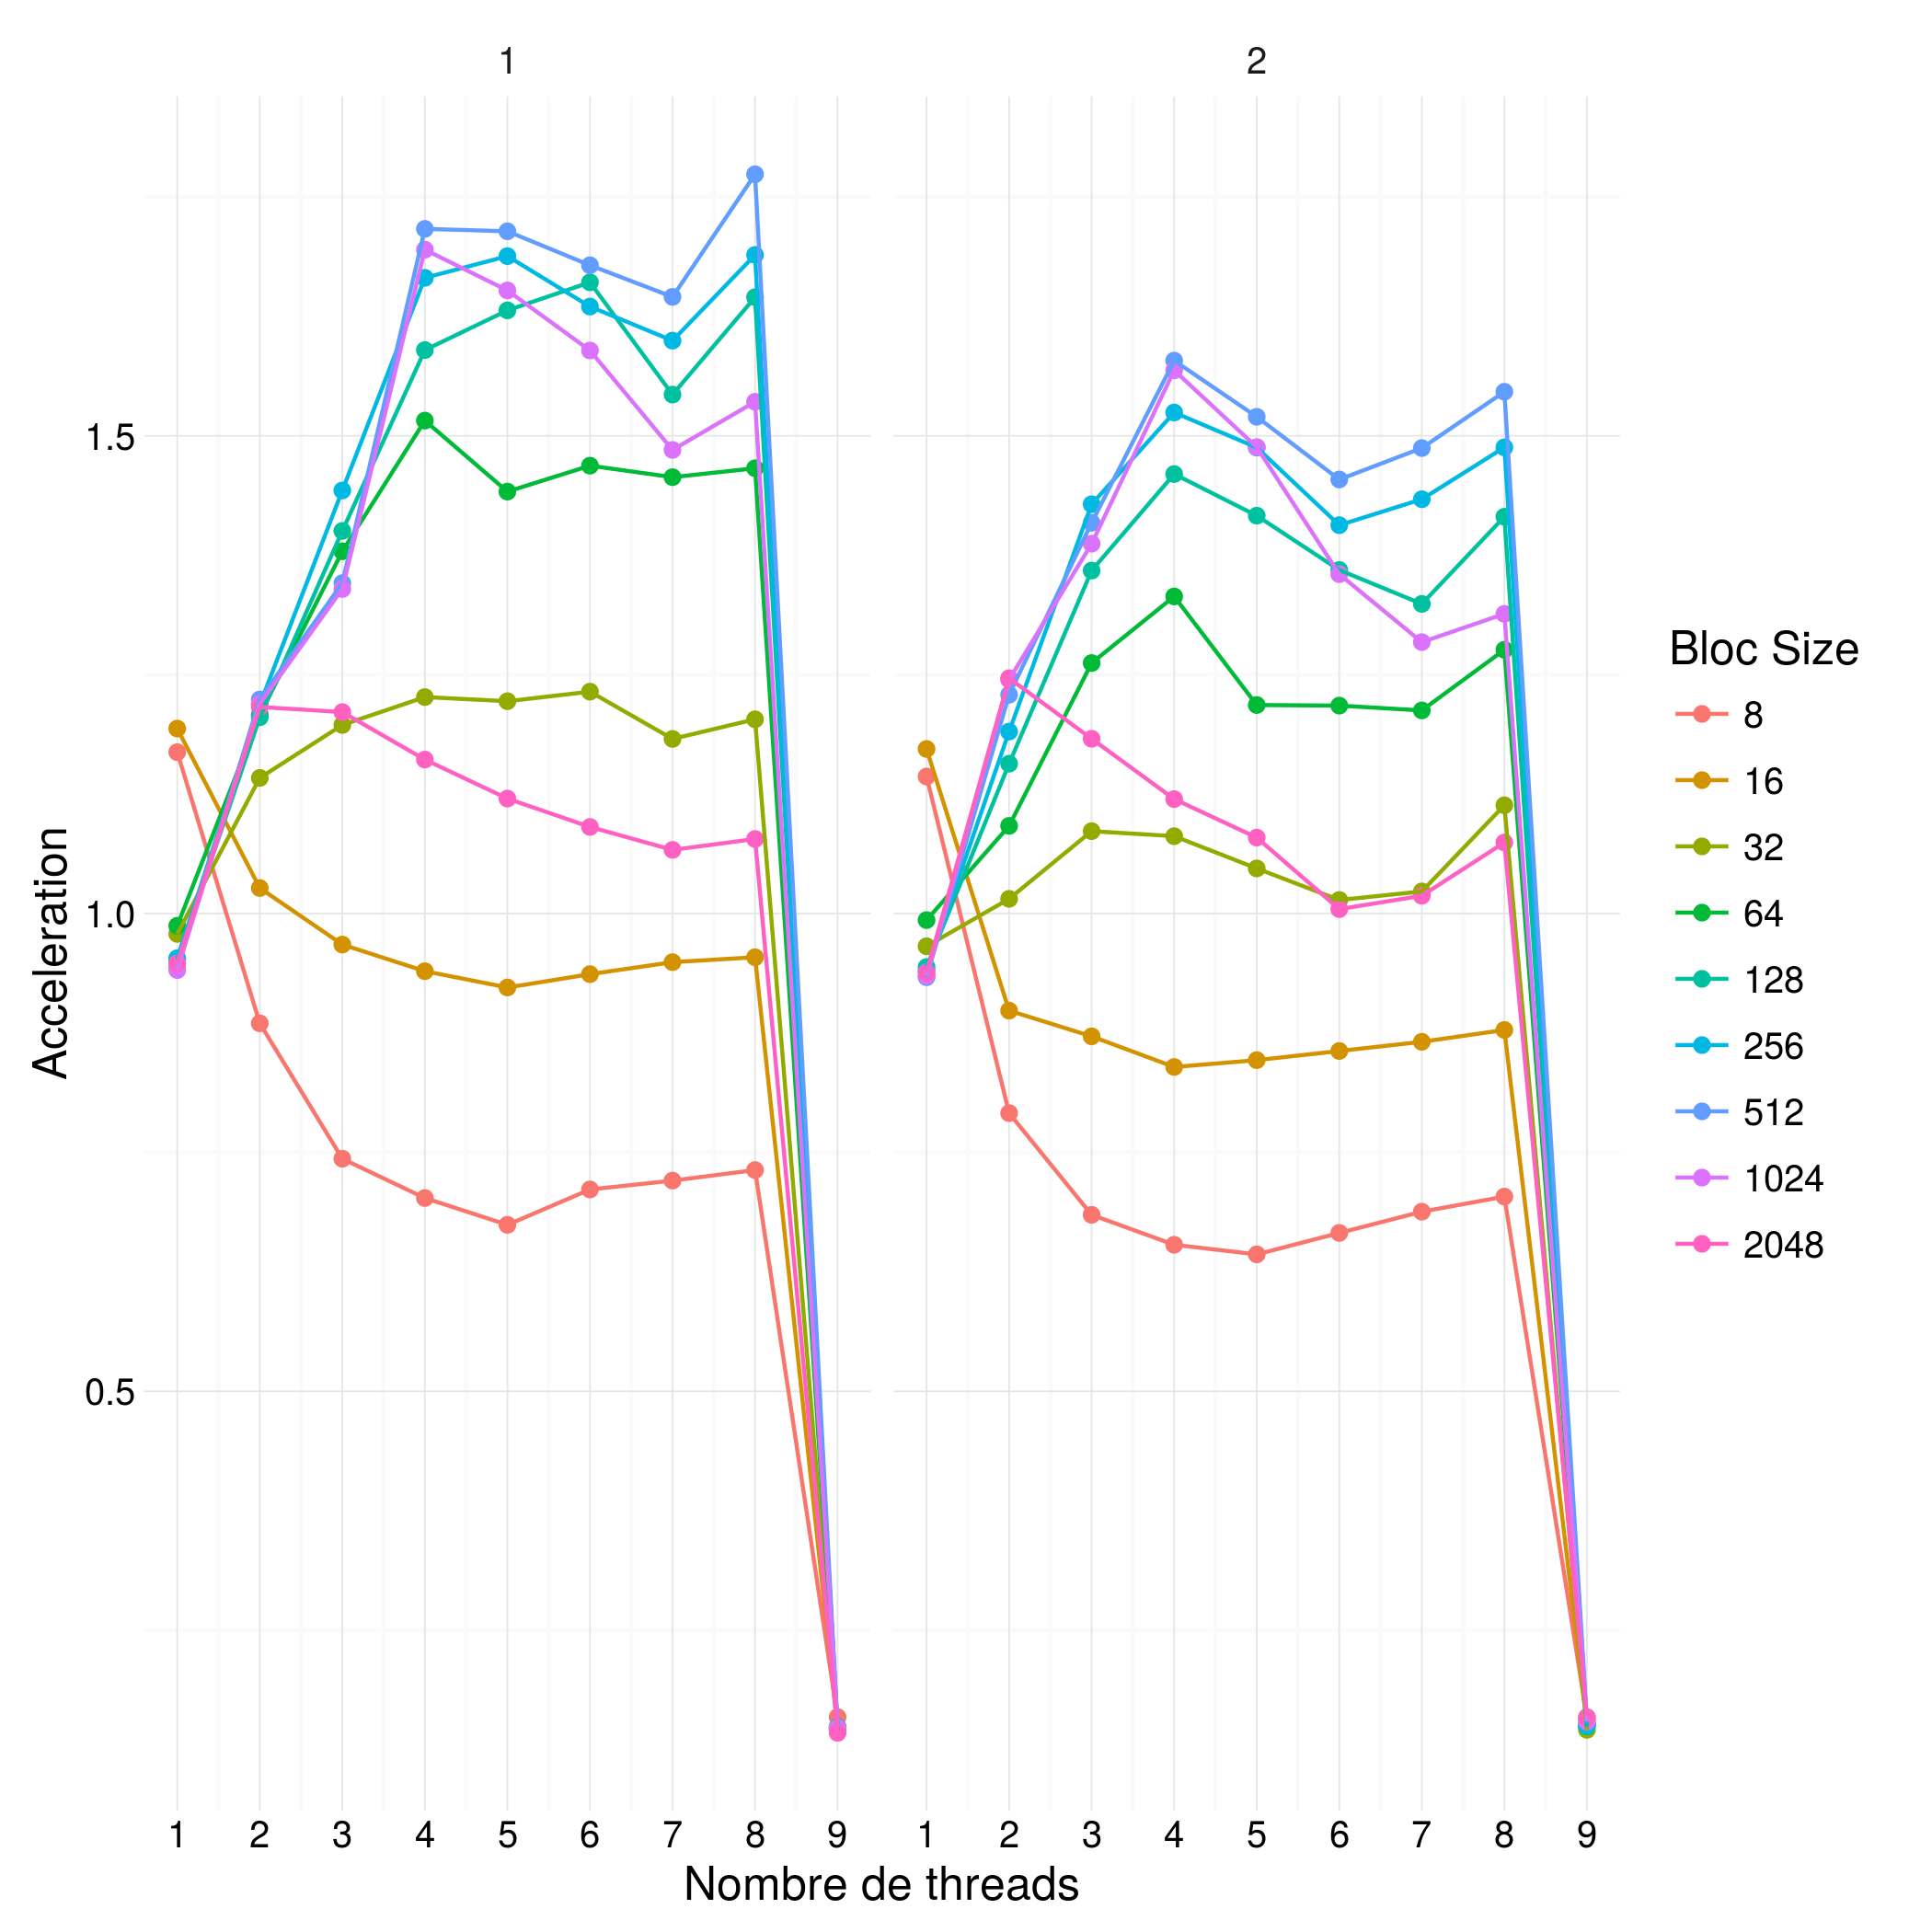
\includegraphics[keepaspectratio,scale=0.5]{./R/Images/Bubble_acell.png}} \\
    \tiny{1: Ordonnancement statique, 2: Dynamique}
  \end{tabular}
\end{center}
A gauche, l' accélération pour un ordonnancement statique et à droite, un ordonnancement dynamique.
On observe que, globalement, pour des paramètres similaires l'ordonnancement dynamique donne de moins bonnes
performances que l'ordonnancement statique avec des allures générales des courbes semblables.
La meilleure performance est obtenue pour 8 threads et des blocs de taille 512.
Intuitivement c'est bien le résultat attendu. Notre tableau est de taille 4096 et en le divisant en huit blocs
(de taille 512) on se dit qu'on pourra tirer parti au mieux des huit coeurs de calcul de notre processeur en affectant le
travail de chaque bloc sur un coeur. Les mesures ci-dessus confirment bien cette intuition.
On voit aussi ici que l'hyperthreading ne fonctionne pas bien pour notre application. Au delà de huit threads les performances s'effondrent.





\section{Tri fusion}
Nous nous intéressons aux gains de performances obtenues par parallélisation du tri par fusion.
Notre étude porte sur le code suivant:
 \begin{minted}[breaklines, numbersep=5pt, gobble=2, frame = lines, framesep=2mm]{c}
   void sort(int *T, unsigned int debut, unsigned int fin){
     #pragma omp parallel num_threads(nb_thread)
     #pragma omp master
     {
       parallel_merge_sort(T, debut, fin);
     }
   }
   
   void parallel_merge_sort(int *T, unsigned int debut, unsigned int fin)
   {
     if (debut < fin) {
       /* si le tableau à trier est petit on le trie
          avec une version séquentielle de merge_sort */
       if ((fin - debut) <= threshold) {
         merge_sort(T, debut, fin);
       } else {
         unsigned int milieu = (fin + debut) / 2;

         /* partie gauche */
         #pragma omp task
         parallel_merge_sort(T, debut, milieu);

         /* partie droite */
         #pragma omp task
         parallel_merge_sort(T, milieu + 1, fin);

         /* merge des deux parties du tableau */
         #pragma omp taskwait
         merge(T, debut, milieu, fin);
       }
     }

     return;
   }
 \end{minted}
 \subsection{Nombre de tâches crées}
 Soit \texttt{T} un tableau de taille $N=2^n$ à trier.
 Avec l'algorithme proposé dans l'énoncé, lors de la division du tableau en deux sous-parties de tailles égales,
 chaque partie est affectée à une nouvelle tâche. On peut représenter les opérations successives de divisions
 par un arbre binaire complet:
 \begin{lstlisting}[basicstyle={\scriptsize\ttfamily}, columns={fixed}, frame={}]
                  N                : 1 noeud
            .     .     .               .
          .       .       .             .
        .         .         .           .
       4          4          4     : N/4 noeuds
     /   \      /   \   ...   \
     2         2               2   : N/2 noeuds
   /   \     /   \           /   \
   1   1 ... 1   1   ...     1   1 : N feuilles
 \end{lstlisting}
 Chaque noeud de l'arbre représente une tâche affectée au tri d'un sous-tableau dont la taille est l'étiquette du noeud.
 Le nombre de noeuds de l'arbre est 
 $$ \sum_{k=0}^{n} N * 2^{-k} $$
 et sa hauteur est $log_2(N)=n$.

 \subsection{Seuil}
 Afin de limiter le nombre de tâches crées, nous proposons d'introduire un seuil (\texttt{threshold}) pour la taille des sous-tableaux. Lorsqu'un tableau à trier est de taille inférieure à ce seuil on effectue le tri avec une version
 séquentielle de l'algorithme. Ainsi on ne parallélise que le tri des noeuds en haut de l'arbre.
 \begin{lstlisting}[basicstyle={\scriptsize\ttfamily}, columns={fixed}, frame={}]
                  N                : 1 noeud
            .     .     .               .
          .       .       .             .            Tri parallèle
        .         .         .           .
       4          4          4     : N/4 noeuds
---------------------------------------------------- Seuil                   
     /   \      /   \   ...   \
     2         2               2   : N/2 noeuds      Tri séquentiel
   /   \     /   \           /   \
   1   1 ... 1   1   ...     1   1 : N feuilles
 \end{lstlisting} 

\subsection{Accélération}
Nous mesurons le temps de tri de tableaux de tailles allant de $2^{13}$ à $2^{18}$. Pour calculer l'accélération, pour chaque
triplet (\texttt{nb\_thread}, \texttt{taille\_tableau}, \texttt{threshold}) nous prenons pour référence le temps moyen d'exécution séquentielle du tri par fusion pris sur 100 expériences.
Nous observons ici l'influence de la taille du seuil sur l'accélération. Au dessus de chaque graphique est indiqué
le seuil utilisé pour les mesures.
\begin{center}
  \begin{tabular} {c}
    \raisebox{-.5\height}{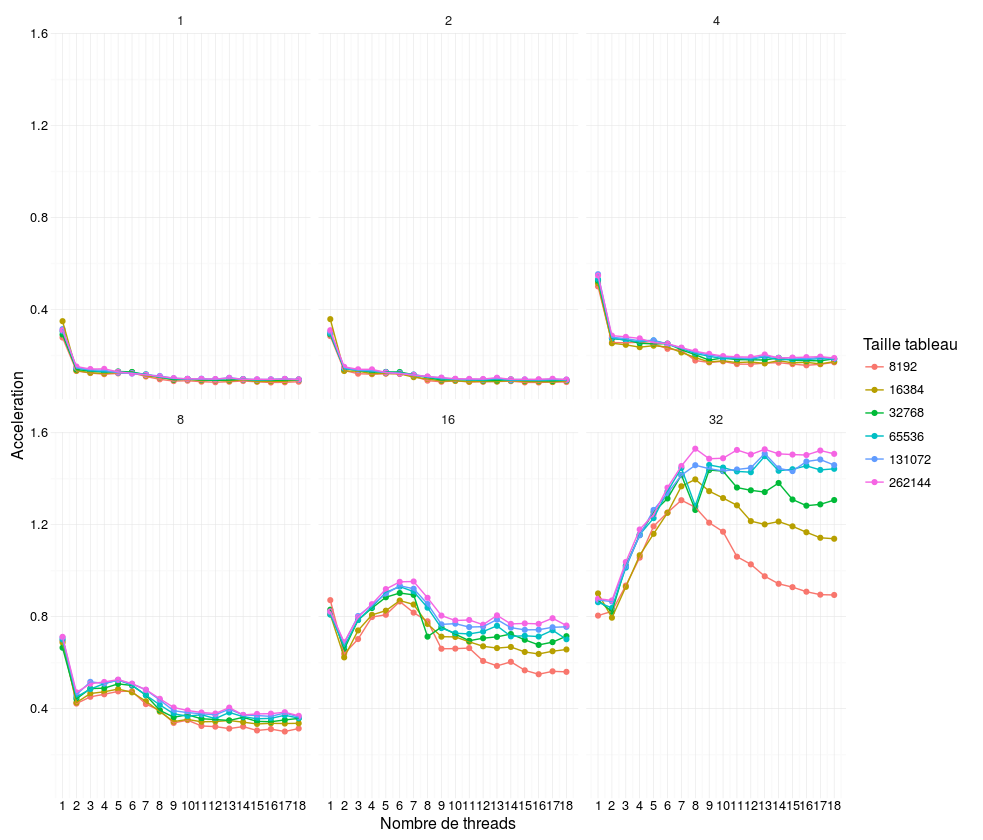
\includegraphics[keepaspectratio,scale=0.5]{./R/Images/Merge_acell_small_threshold.png}}
  \end{tabular}
\end{center}

En haut à gauche, on observe que pour la version naïve de l'algorithme, avec une tâche pour chaque sous-tableau, on obtient des performances beaucoup moins bonnes que la version séquentielle.
Les premiers gains commencent à apparaître avec un seuil égal à 32 (en bas à droite).
On poursuit notre expérimentation avec des seuils plus grands.
\begin{center}
  \begin{tabular} {c}
    \raisebox{-.5\height}{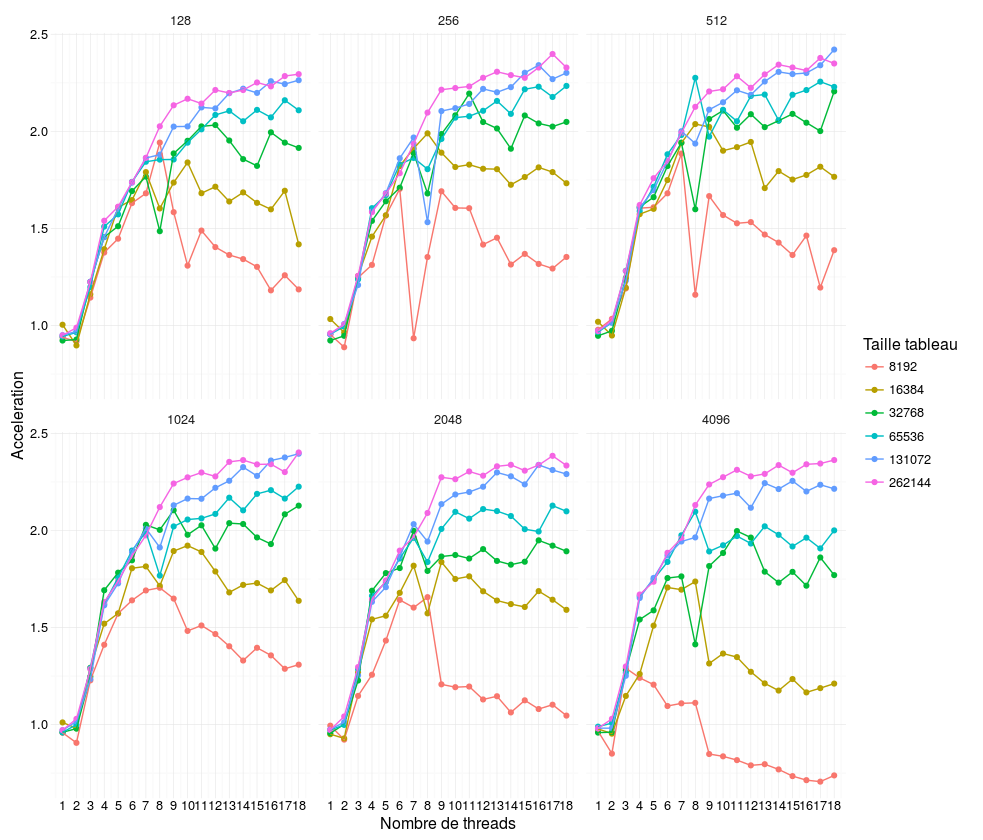
\includegraphics[keepaspectratio,scale=0.5]{./R/Images/Merge_acell.png}}
  \end{tabular}
\end{center}
On observe que si l'on dimensionne correctement la valeur du seuil, on arrive à obtenir
un facteur 2.5 d'accélération. Intuitivement on voit que prendre un seuil trop proche de la taille du tableau à trier
revient à faire majoritairement du séquentiel, et prendre un seuil trop petit revient à paralléliser inutilement.
On perçoit avec notre algorithme une nette amélioration des performances du tri fusion.
Intuitivement nous ne pensions pas obtenir de si bon résultats en raison des opérations de fusion
s'effectuant en séquentiel. Nous sommes donc très satisfait de notre choix.

\section{Conclusion}
Ce travail constituait une première expérience avec \texttt{OpenMP}.
Nous avons pû confronter nos intuitions sur les gains de performances à des mesures et une étude statistique concrète.
Nous avons apprécié la simplicité de mise en oeuvre du parallélisme avec \texttt{OpenMP} et l'efficacité du langage \texttt{R}
pour l'analyse statistique de nos résultats expérimentaux.

\section{Annexe}
\subsection{Conditions expérimentales}

\subsubsection {Infos Cpu}
la commande \texttt{lscpu} permet d'afficher les informations liées aux processeurs.
\begin{lstlisting}[columns=fixed,basicstyle=\scriptsize\ttfamily]
Architecture :                           x86_64
Mode(s) opératoire(s) des processeurs :  32-bit, 64-bit
Boutisme :                               Little Endian
Processeur(s) :                          8
Liste de processeur(s) en ligne :        0-7
Thread(s) par cœur :                     2
Cœur(s) par socket :                     4
Socket(s) :                              1
Nœud(s) NUMA :                           1
Identifiant constructeur :               GenuineIntel
Famille de processeur :                  6
Modèle :                                 94
Nom de modèle :                          Intel(R) Core(TM) i7-6700 CPU @ 3.40GHz
Révision :                               3
Vitesse du processeur en MHz :           799.987
Vitesse maximale du processeur en MHz :  4000,0000
Vitesse minimale du processeur en MHz :  800,0000
BogoMIPS :                               6818.00
Virtualisation :                         VT-x
Cache L1d :                              32K
Cache L1i :                              32K
Cache L2 :                               256K
Cache L3 :                               8192K
Nœud NUMA 0 de processeur(s) :           0-7
Drapaux :                                fpu vme de pse tsc msr pae mce cx8 apic sep mtrr pge mca cmov pat pse36 clflush dts acpi mmx fxsr sse sse2 ss ht tm pbe syscall nx pdpe1gb rdtscp lm constant_tsc art arch_perfmon pebs bts rep_good nopl xtopology nonstop_tsc cpuid aperfmperf tsc_known_freq pni pclmulqdq dtes64 monitor ds_cpl vmx smx est tm2 ssse3 sdbg fma
cx16 xtpr pdcm pcid sse4_1 sse4_2 x2apic movbe popcnt tsc_deadline_timer aes xsave avx f16c rdrand lahf_lm abm 3dnowprefetch cpuid_fault intel_pt tpr_shadow vnmi flexpriority ept vpid fsgsbase tsc_adjust bmi1 hle avx2 smep bmi2 erms invpcid rtm mpx rdseed adx smap clflushopt xsaveopt xsavec xgetbv1 xsaves dtherm ida arat pln pts hwp hwp_notify hwp_act_window hwp_epp
\end{lstlisting}

\subsection {Info Mémoire}
Nous récupérons les informations concernant la mémoire avec la commande \texttt{sudo lshw}
\begin{lstlisting}[columns=fixed,basicstyle=\scriptsize\ttfamily]
 description: Mémoire Système
       identifiant matériel: 41
       emplacement: Carte mère
       taille: 32GiB
     *-bank:0
          description: DIMM DDR4 Synchrone 2133 MHz (0,5 ns)
          produit: CMK32GX4M2A2133C13
          fabriquant: AMI
          identifiant matériel: 0
          numéro de série: 00000000
          emplacement: ChannelA-DIMM0
          taille: 16GiB
          bits: 64 bits
          horloge: 2133MHz (0.5ns)
     *-bank:1
          description: DIMM DDR4 Synchrone 2133 MHz (0,5 ns)
          produit: CMK32GX4M2A2133C13
          fabriquant: AMI
          identifiant matériel: 1
          numéro de série: 00000000
          emplacement: ChannelA-DIMM1
          taille: 16GiB
          bits: 64 bits
          horloge: 2133MHz (0.5ns)
\end{lstlisting}

\end{document}
